% !TeX root = ../thuthesis-example.tex

\chapter{交互式手语学习助手设计与实现}
手语是听障人士进行交流的主要方式。然而,由于手语学习资源有限、学习成本高等原因,听障人士与普通人之间存在较大的交流障碍。随着人工智能技术的发展,基于计算机视觉的手语识别与生成技术为解决这一问题提供了新的可能。本章将基于前文提出的多策略解耦和语义集成网络(MDSI)以及协同手势生成算法(CoordSpeaker),设计并实现一个交互式手语学习助手系统。该系统旨在为手语学习者提供实时的动作评估与反馈,帮助提升手语学习效果。

\section{系统总体设计}

\subsection{设计目标}
本系统旨在通过人工智能技术辅助手语学习过程,为学习者提供实时、准确的动作评估与反馈。系统的核心目标是实现高效的手语学习体验,这要求系统具备实时的动作识别能力和自然的人机交互界面。基于这一目标,系统需要在准确性、实时性、交互性和适应性等多个维度上达到较高水平。
在准确性方面,系统基于本文提出的MDSI算法,通过多模态特征的解耦与融合实现高精度的手语动作识别。该算法能够有效处理手语动作中的细微差异,为学习评估提供可靠的技术支持。
在实时性方面,系统采用并行计算技术,确保手语动作的捕获、识别和反馈过程能够实时完成,从而保证良好的交互体验。
在交互性方面,系统设计了直观的可视化界面,通过实时对比展示标准动作与用户动作的差异,并结合定量评估指标提供针对性的改进建议。在适应性方面,系统支持根据用户的学习进度和掌握程度动态调整练习内容和难度,实现个性化的学习体验。

\subsection{系统架构}
为实现上述设计目标,本系统采用模块化的软件架构设计,如图~\ref{fig:system_arch}所示。系统整体划分为手语识别、手语生成、交互反馈三个核心功能模块,各模块通过统一的消息总线进行通信协作。这种模块化设计不仅提高了系统的可维护性和可扩展性,也便于各个功能模块的独立优化和升级。
手语识别模块作为系统的核心感知单元,负责实时捕获和识别用户的手语动作。该模块基于MDSI算法实现,能够有效处理手语动作中的复杂特征。
手语生成模块则基于CoordSpeaker协同手势生成算法,负责生成标准的手语动作示范,支持基于文本描述的精确控制,为学习者提供准确的参考样本。
交互反馈模块通过比对用户动作与标准动作,实时生成评估结果和改进建议。%该模块采用多维度的评估指标,既关注动作的准确性,也考虑动作的流畅度和节奏感。
% 用户界面模块则通过可视化方式呈现系统功能,提供直观的学习交互体验。


\begin{figure}
    \centering
    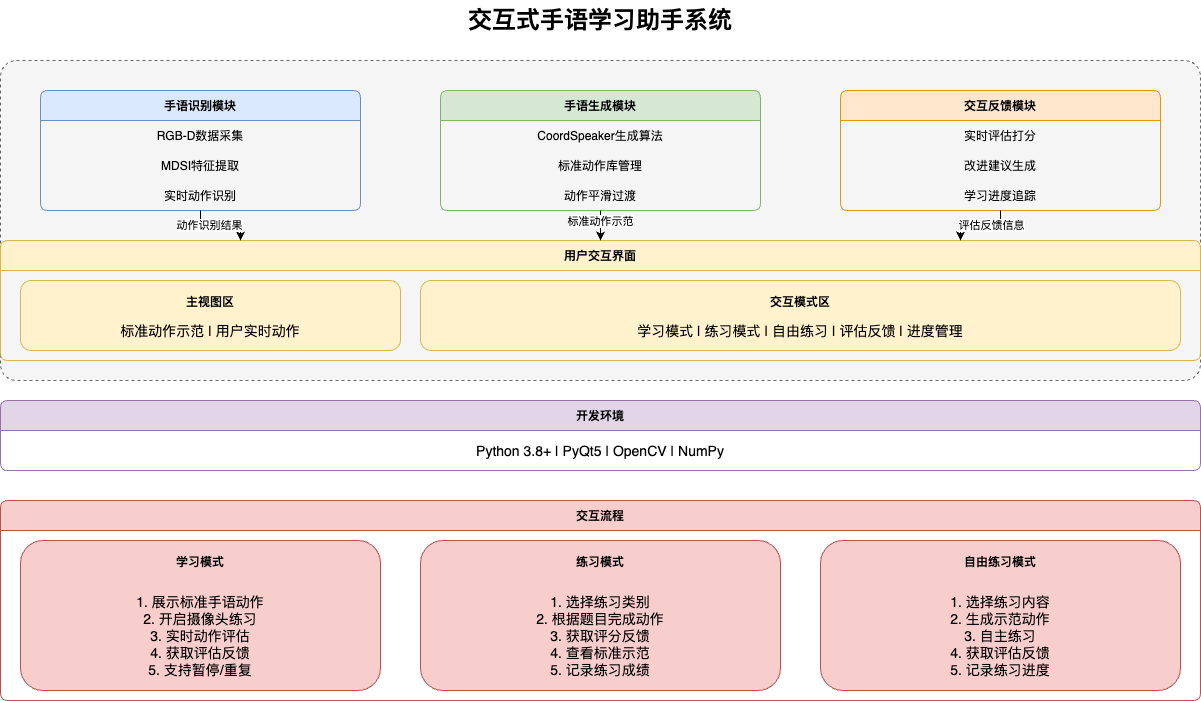
\includegraphics[width=\linewidth]{sys.drawio.png}
    % \caption*{}
    \caption{交互式手语学习助手系统架构}
    \label{fig:system_arch}
  \end{figure}

\section{核心功能模块设计}

\subsection{手语识别模块}
手语识别模块是系统的核心组件之一,负责实时捕获并识别用户的手语动作,进行评估打分。该模块基于第三章提出的MDSI算法,通过RGB-D相机实时采集用户手语动作的RGB图像序列与深度信息。为提升系统实时性能,本模块采用可插拔的高效MDSI算法,基于GPU加速,有效降低了系统延迟。

\subsection{手语生成模块}
手语生成模块负责生成标准手语动作示范,以供学习/练习使用。基于第四章提出的CoordSpeaker协同手势生成算法实现。该模块支持两种工作模式:离线生成模式和实时生成模式。离线生成模式用于预先生成标准动作库,包含常用手语词汇和短语的标准示范动作。实时生成模式则支持根据文本输入即时生成手语动作示范,为用户提供更灵活的学习参考。

\subsection{交互反馈模块}
交互反馈模块通过实时比对用户动作与标准动作,生成评估得分与改进建议。%该模块采用多维度评估体系,包括动作准确度、完整度、流畅度等指标。
系统通过可视化方式直观展示用户动作与标准动作的差异,并结合自然语言描述提供具体的改进建议。此外,模块还会记录用户的学习轨迹,支持学习进度的追踪与分析。


\begin{figure}
    \centering
    \begin{subfigure}[b]{0.7\linewidth}
        \centering
        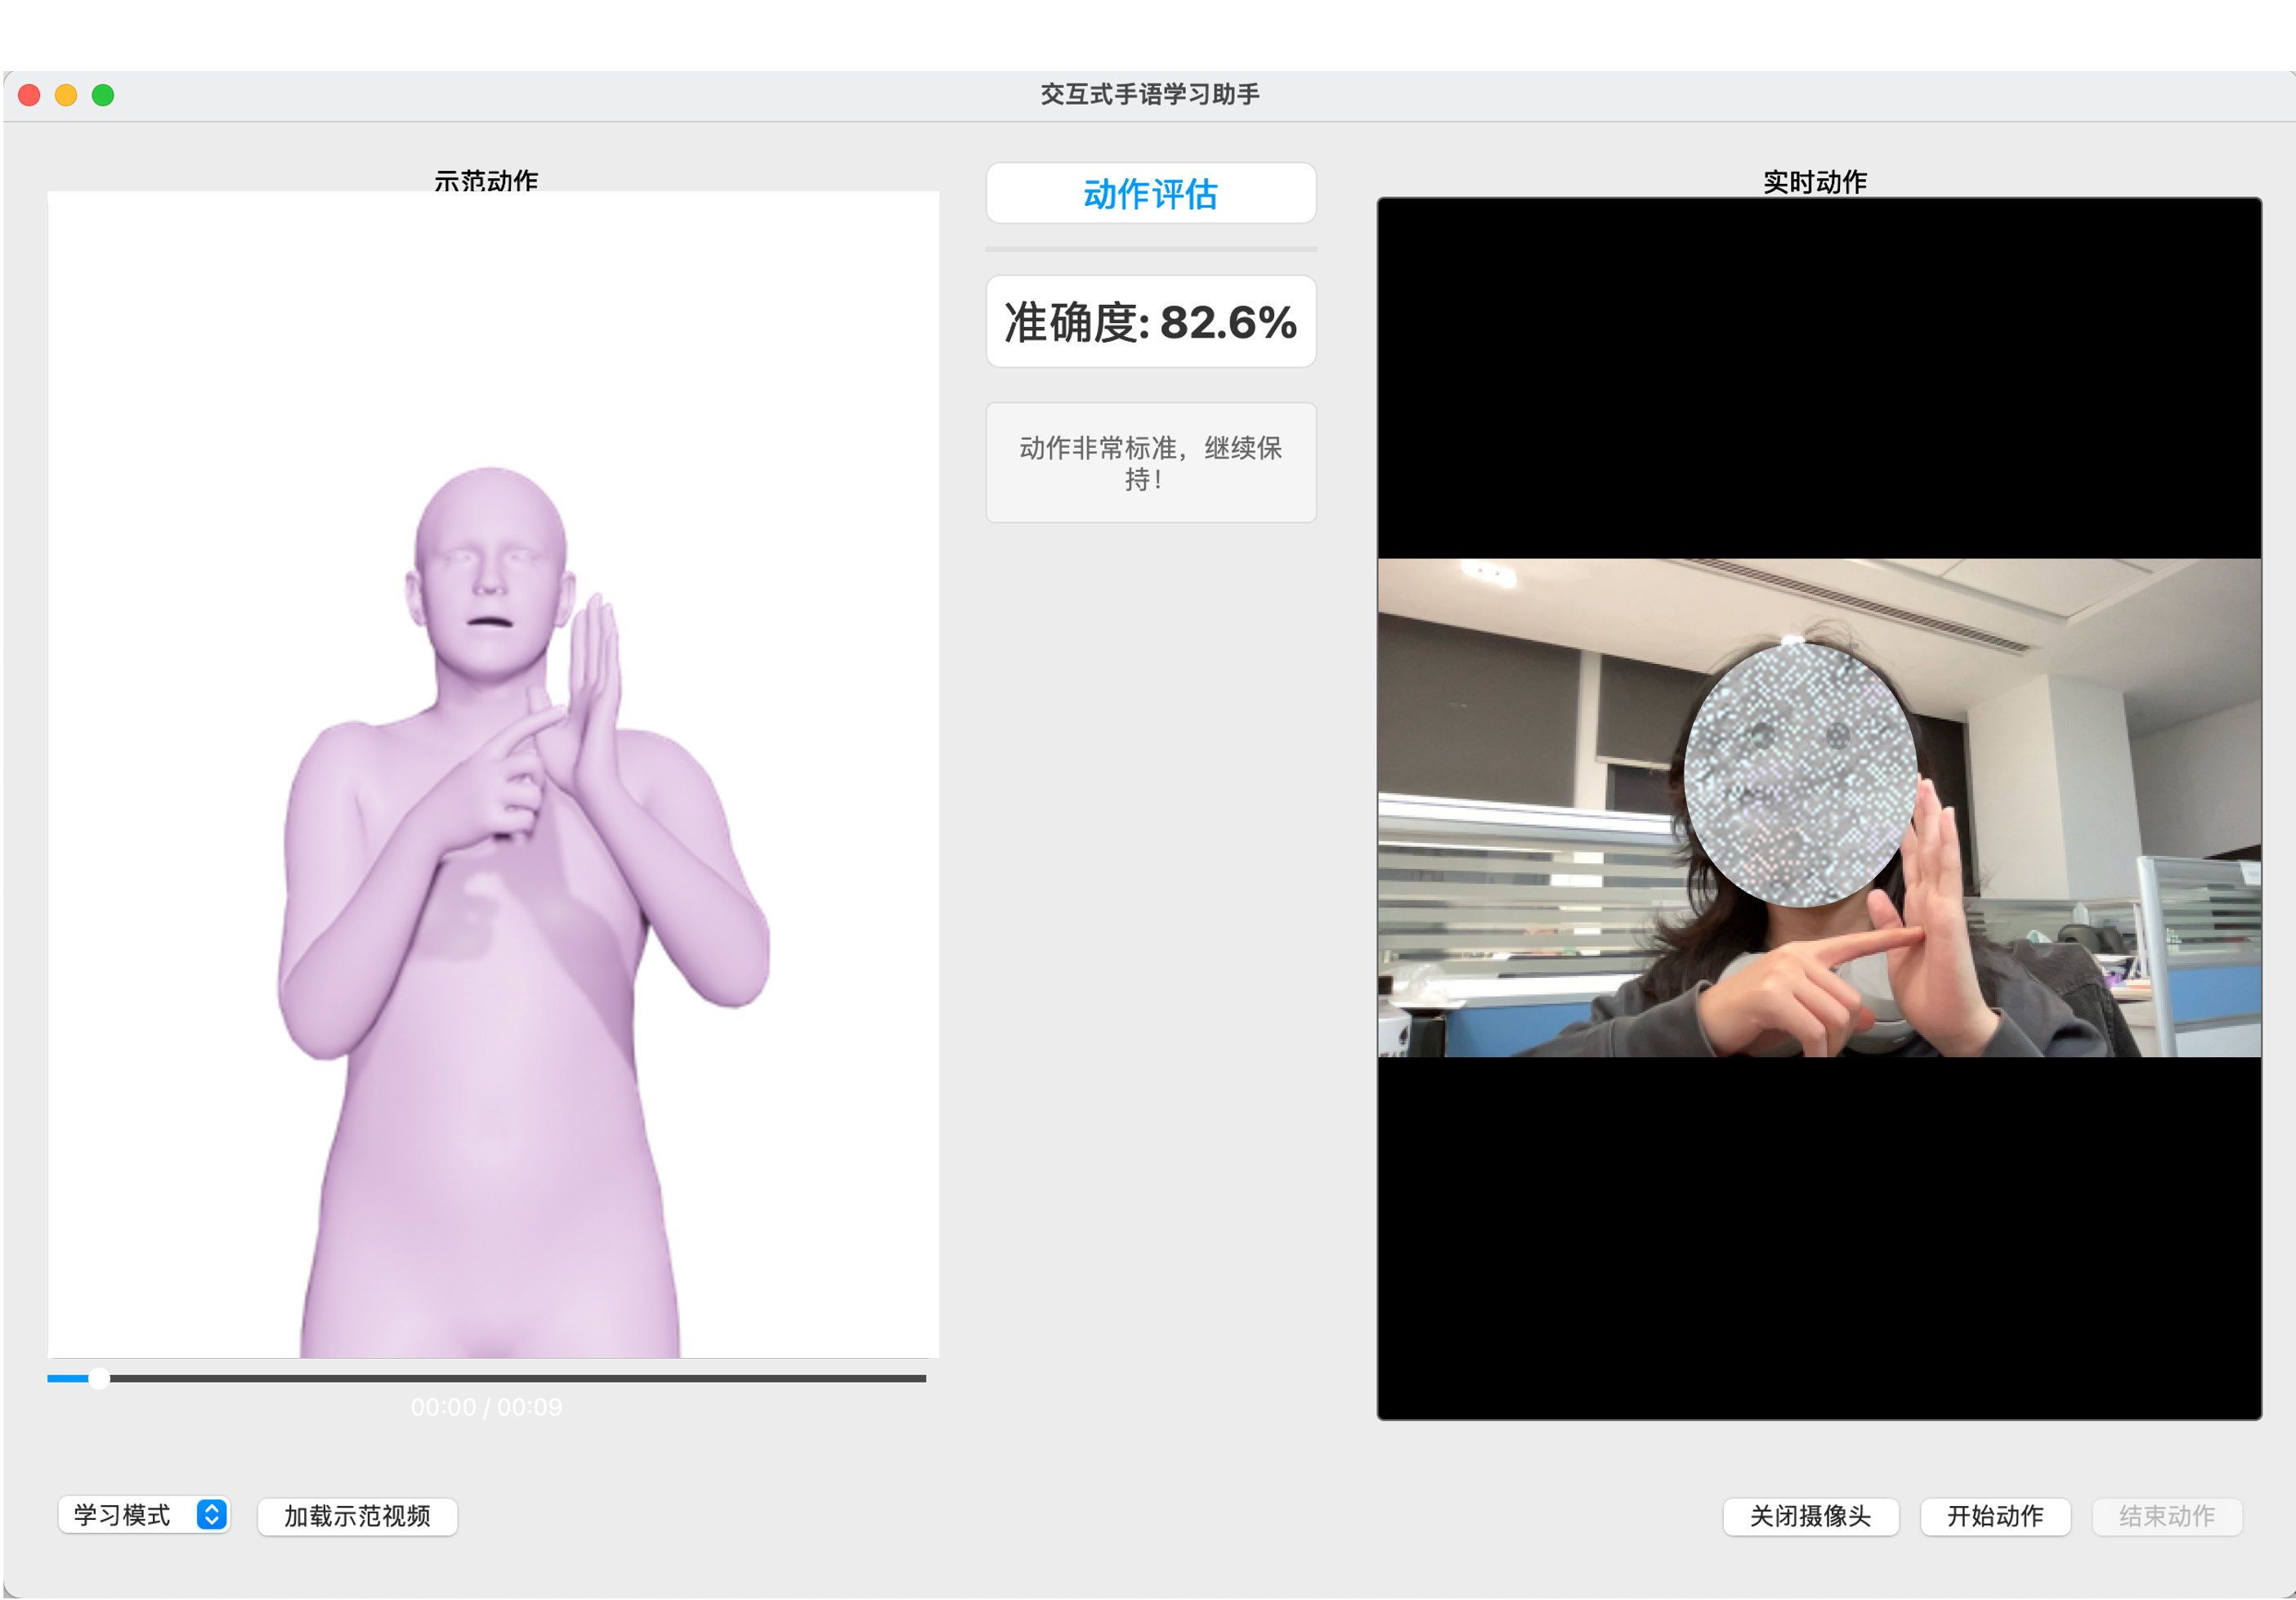
\includegraphics[width=\linewidth]{demo_learn.png}
        \caption{“学习模式”}
    \end{subfigure}
    \hfill
    \begin{subfigure}[b]{0.7\linewidth}
        \centering
        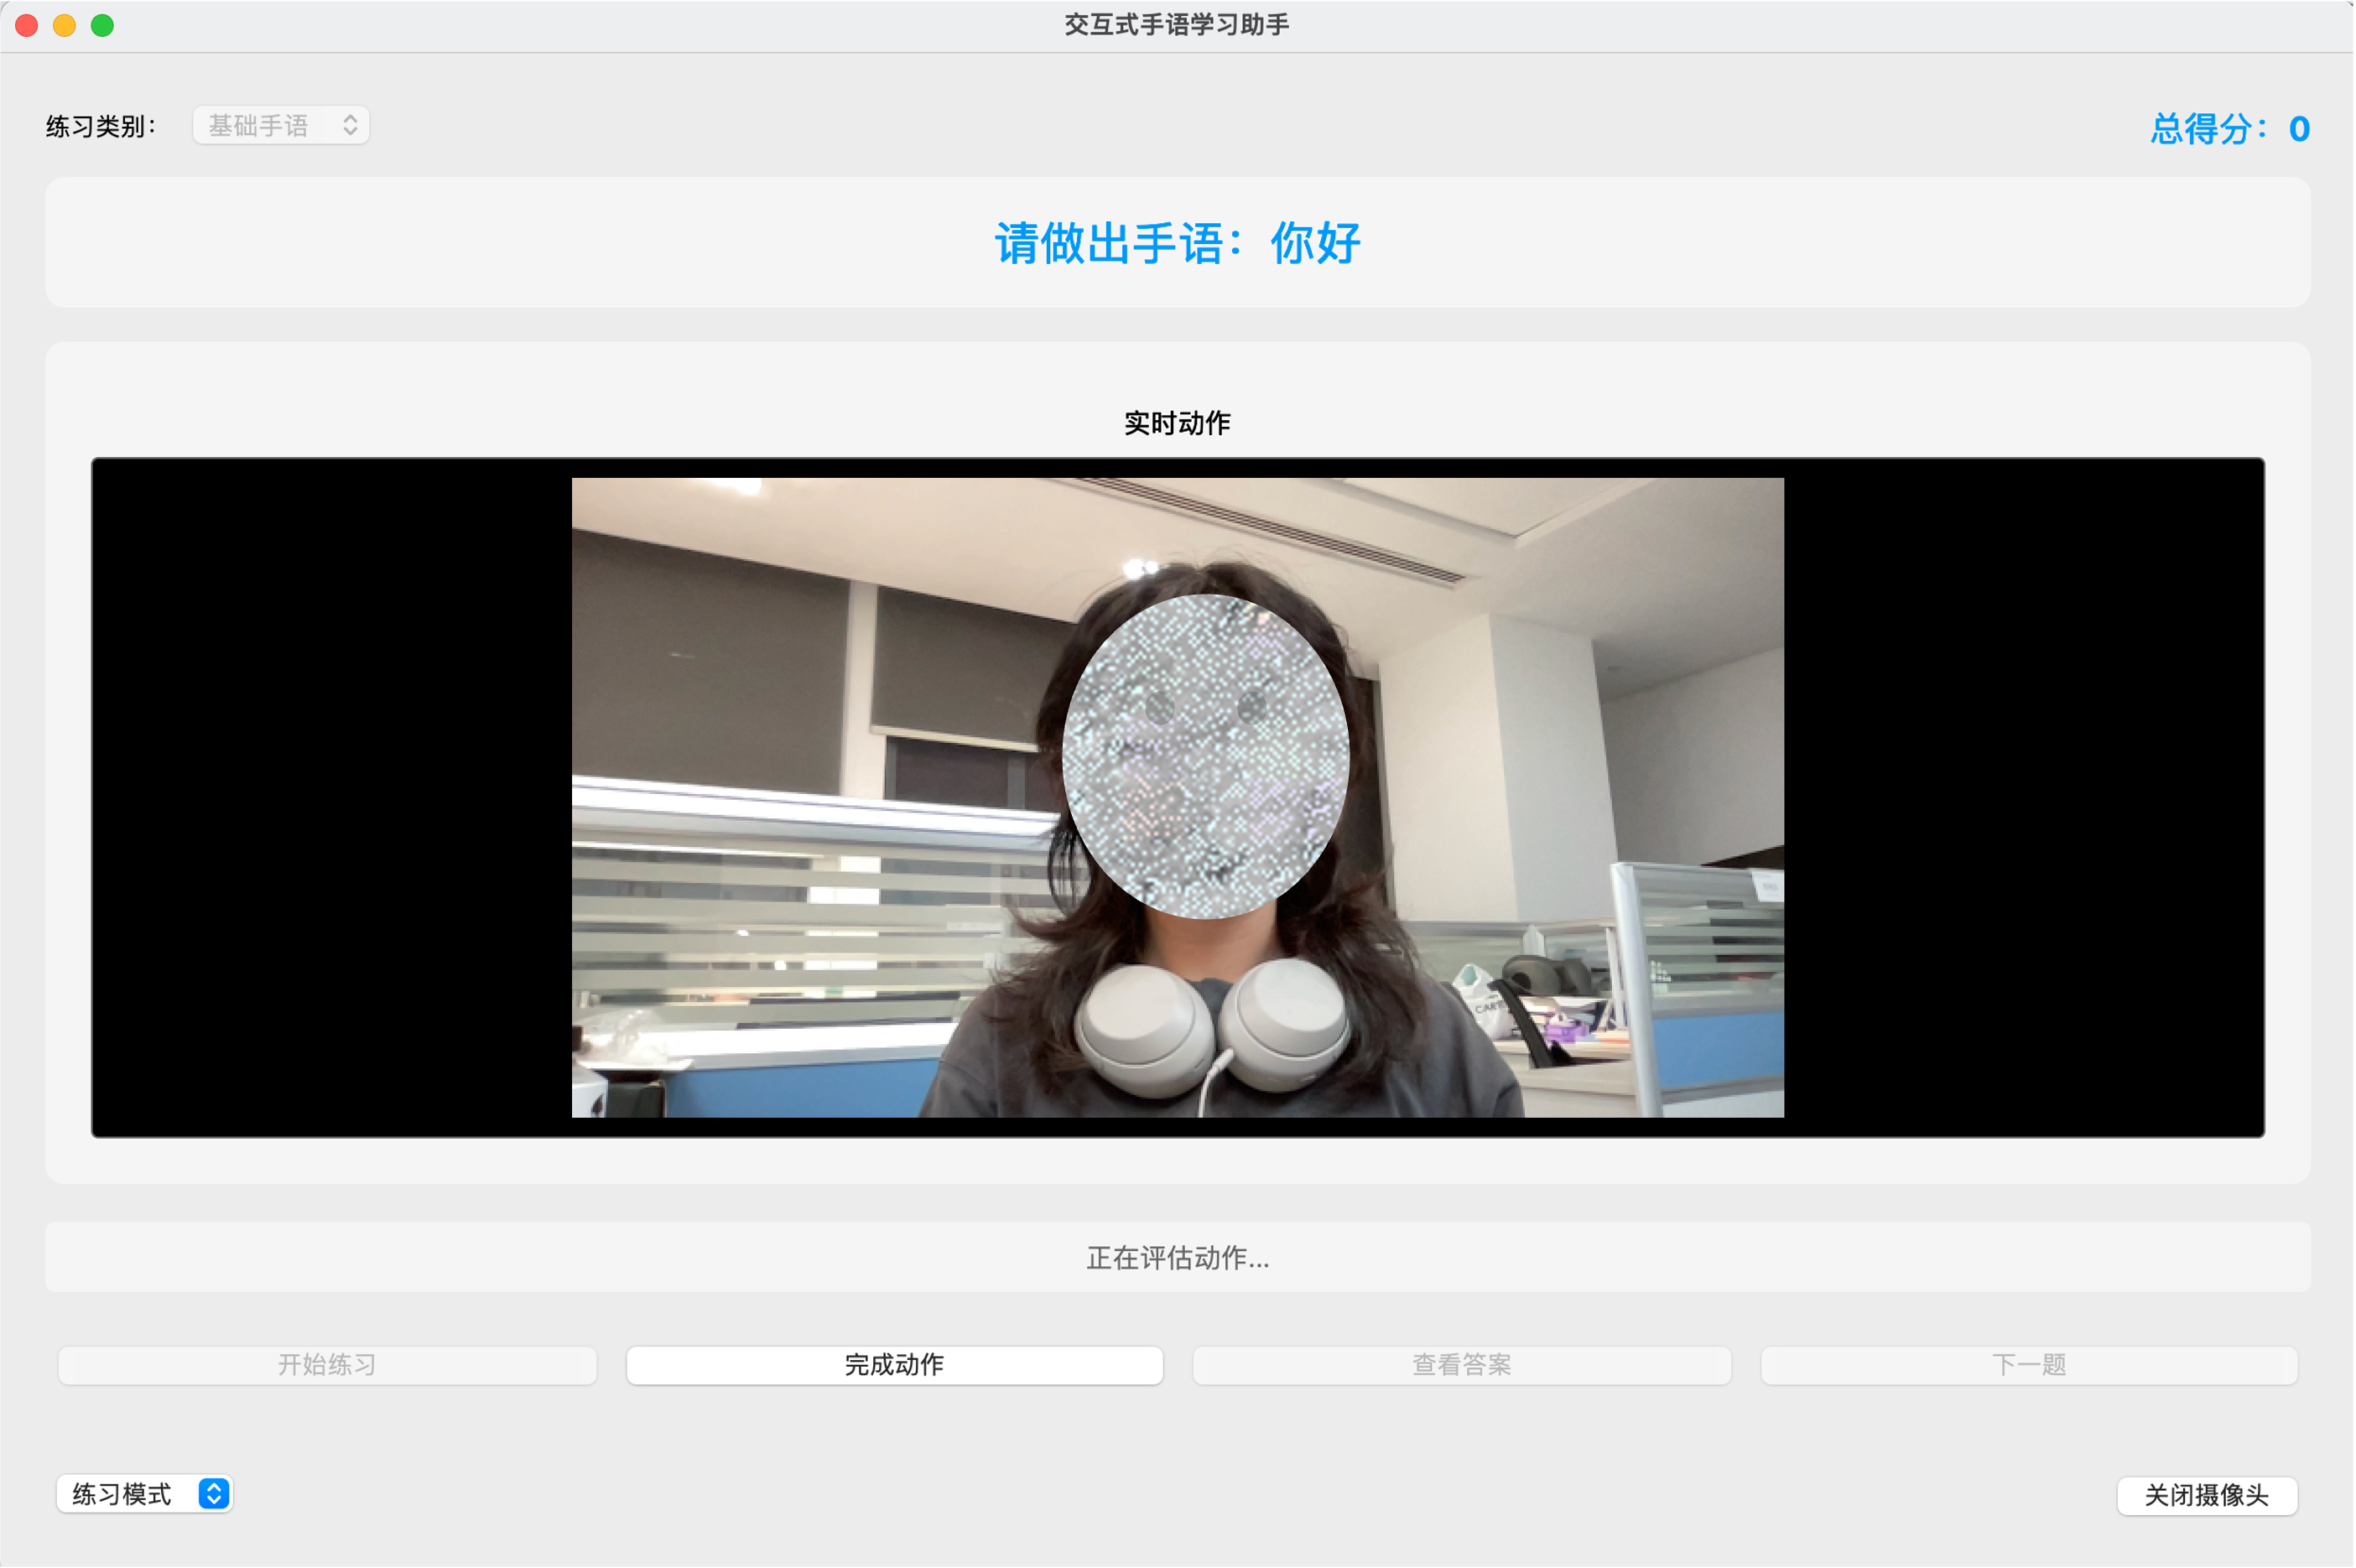
\includegraphics[width=\linewidth]{demo_practice.png}
        \caption{“练习模式”}
    \end{subfigure}
    \caption{用户界面设计}
    \label{fig:ui_design}
\end{figure}
  
\section{人机交互设计}

\subsection{手语学习模式}
系统支持手语学习、练习评估和自由练习三种主要交互模式。在手语学习模式下,系统首先展示标准手语动作示范,用户通过摄像头采集练习动作,系统实时提供评估反馈。练习评估模式则提供多组不同难度系统化的练习题目,用户需要根据题目完成指定手语动作,系统给出评分和改进建议。自由练习模式支持用户自主选择练习手语词汇,系统生成相应的示范动作,供用户自主练习,并给出评估反馈。

\subsection{用户界面设计}
系统界面采用分区布局设计,主要包含主视图区、评估反馈区和功能控制区三个主要部分。以“学习模式”为例(如图~\ref{fig:ui_design}所示):主视图区采用左右分屏布局,左侧显示标准手语动作示范,右侧实时显示用户的动作画面,便于用户直观对比和模仿。评估反馈区位于界面中部,在用户完成当前手语动作后,显示动作评估分数、关键改进建议和动作要点提示。功能控制区则集中展示学习模式选择、难度调节等操作按钮,保证操作的便捷性。练习模式与学习模式类似,区别在于反馈区位于上下,分别显示题目和评估的分数,用户根据题目完成指定手语动作后,系统给出评分和改进建议,用户可进一步查看答案示范。



\subsection{交互引导设计}
如图~\ref{fig:ui_interaction}所示为帮助用户更好地理解系统功能,系统在主界面及各个模式中设计了交互引导功能。当用户首次启动系统时,会显示可选择的学习模式与系统功能。当首次进入子模式时,系统会通过弹窗提示用户进行相关操作,如开启摄像头,并引导用户进行手语学习。在手语学习过程中,系统支持用户根据的学习进度和掌握程度,自主调整练习内容和难度,确保用户能够持续进步。

\begin{figure}
    \centering
    \begin{subfigure}[b]{0.48\linewidth}
        \centering
        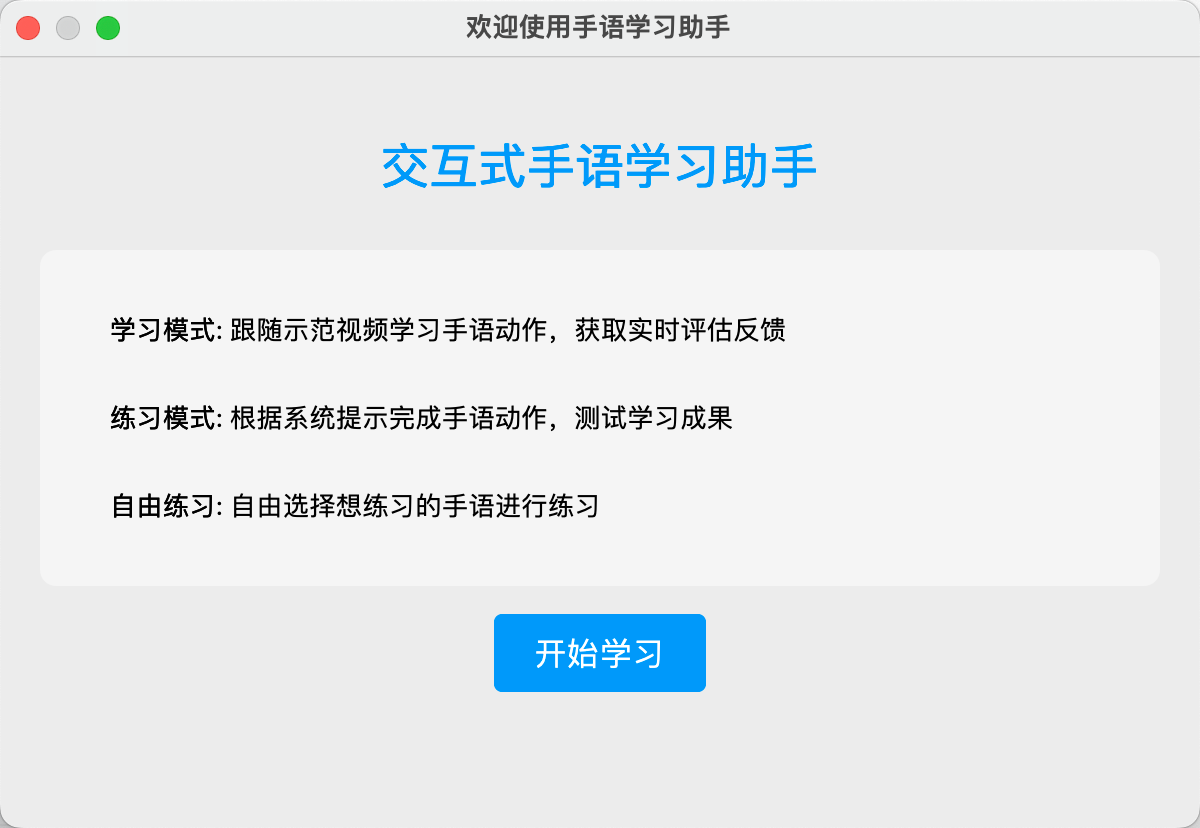
\includegraphics[width=\linewidth]{demo_main.png}
        \caption{“主界面”}
    \end{subfigure}
    \hfill
    \begin{subfigure}[b]{0.48\linewidth}
        \centering
        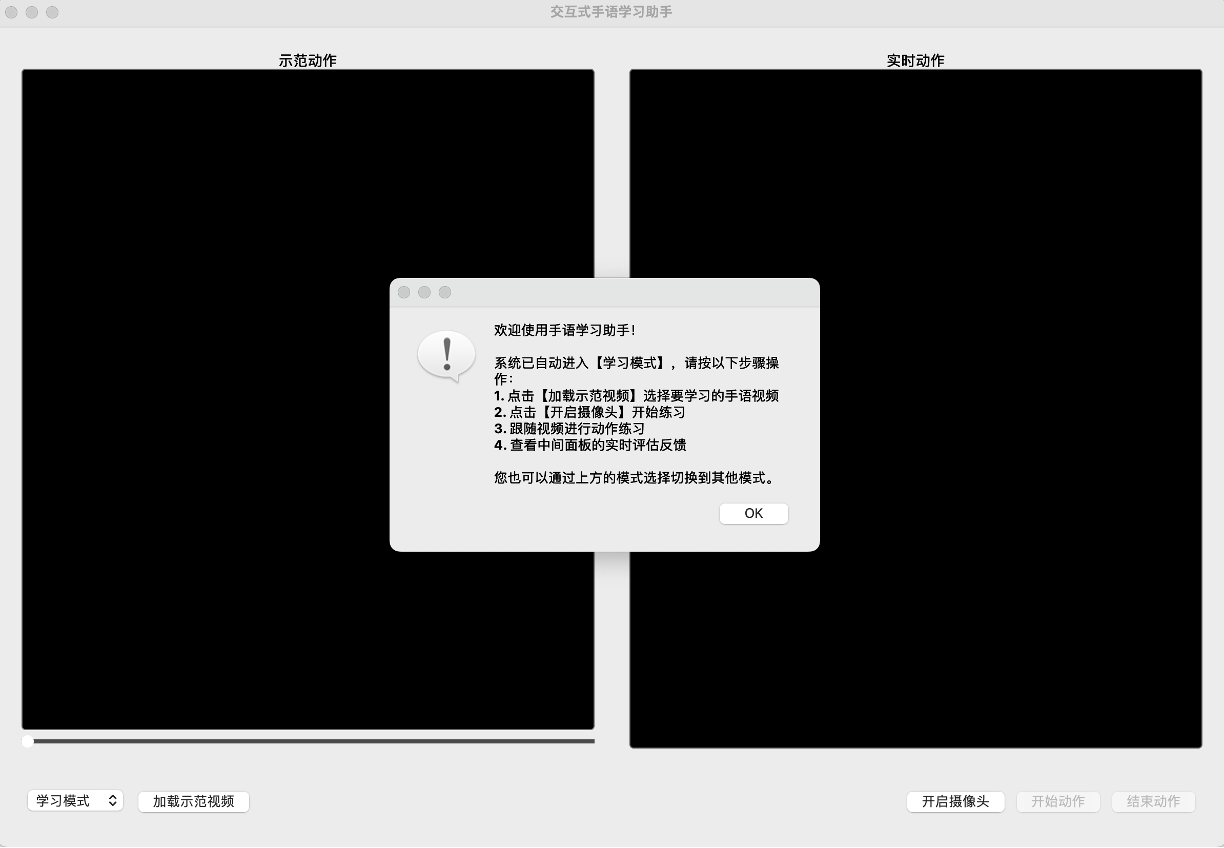
\includegraphics[width=\linewidth]{demo_popup.png}
        \caption{“弹窗引导”}
    \end{subfigure}
    \caption{交互引导设计}
    \label{fig:ui_interaction}
  \end{figure}

\section{系统实现与部署}
\subsection{开发环境与技术栈}
本系统采用Python作为主要开发语言,基于PyQt5构建图形用户界面。系统的核心算法模块采用PyTorch深度学习框架实现,通过CUDA加速实现GPU并行计算。系统开发环境和主要依赖包括:Python 3.13、PyQt5 5.15、OpenCV 4.11等。
在系统架构方面,采用基于消息队列的模块间通信机制,确保各功能模块之间的解耦与协同。系统部署采用容器化方案,使用Docker实现环境隔离与快速部署。为保证系统的实时性能,手语识别与生成模块均采用GPU加速,并通过多线程技术实现并行执行。

\subsection{关键技术实现}
系统的关键技术实现主要包括以下几个方面:
首先,在手语动作捕获方面,系统通过OpenCV实现RGB-D相机的实时数据采集,采用多线程技术将数据采集与处理解耦,有效降低系统延迟。
其次,在实时手语识别方面,系统基于MDSI算法实现了高效的特征提取与动作识别。
在手语动作生成方面,系统实现了基于CoordSpeaker协同手势生成算法的动作合成引擎。通过预计算与缓存机制,系统显著降低了动作生成的延迟。同时,实现了动作平滑过渡算法,确保生成动作的连贯性与自然性。
在交互反馈方面,系统基于MDSI算法实现了高效准确的手语动作评估,通过分类置信度实时给出评估得分,并基于CoordSpeaker算法生成参考动作答案,同时给出改进建议与学习激励。同时支持学习进度追踪,用户可查看历史学习记录,并根据进度调整学习计划。%设计了基于多特征的评估算法,综合考虑手部位置、运动轨迹、动作速度等因素,实现准确的动作评估。系统采用可视化技术直观展示评估结果,通过骨架对比方式突出动作差异。

    % - 手语识别准确性测试
    % - 手语生成质量评估
    % - 交互响应时间测试
    % - 系统稳定性测试
    % ### 实验设计
    %     - **参与者**:招募10名志愿者,均为手语初学者
    %     - **任务设计**:
    %     1. 基础手语词汇学习(10个常用手语词汇)
    %     2. 简单手语句子练习(5个日常用语)
    %     - **评估指标**:
    %     - 学习效率:完成学习任务所需时间
    %     - 识别准确率:系统识别用户手语动作的准确程度
    %     - 用户满意度:基于问卷的主观评分(1-5分)
    %     - 系统可用性:基于SUS量表的评估


\section{系统测试与评估}
% \subsection{系统功能测试}
% 系统功能测试主要针对手语识别准确性、手语生成质量、交互响应时间和系统稳定性四个方面展开。在手语识别准确性测试中,我们采用标准测试集评估系统的识别性能。测试结果表明,\textcolor{red}{系统在10类常用手语词汇识别任务上达到了99\%以上的准确率。}
% 在手语生成质量评估中,\textcolor{red}{我们邀请专业手语教师对系统生成的标准动作进行评估。评估结果显示,系统生成的手语动作在准确性、流畅性和自然度方面均获得了较高评价。}
% 交互响应时间测试结果表明,\textcolor{red}{系统的端到端延迟控制在100ms以内,满足实时交互需求。}
% 系统稳定性测试采用持续运行方式进行,在24小时连续运行测试中,系统未出现崩溃或性能显著下降的情况,展现了良好的稳定性。
\begin{figure}
    \centering
    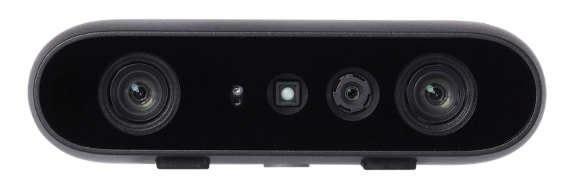
\includegraphics[width=0.7\textwidth]{gemini2.png}
    \caption{奥比中光RGB-D视觉传感器Gemini 2正视实物图。}
    \label{fig:aobi_robot}
  \end{figure}
\paragraph{识别准确率}
为了评估系统的识别准确性,我们使用商业级奥比中光RGB-D相机(图~\ref{fig:aobi_robot})构建了自采数据集,并基于此评估了我们的方法。%本实验共召集\textcolor{red}{xx}名志愿者
共采集了12类数据,每类包含25个样本(图~\ref{fig:aobi_sample})。%参与数据采集的志愿者共计。%均来自xxx,涵盖不同性别、年龄及手势习惯,以确保数据的多样性与代表性。
采集过程遵循\cite{wan2016chalearn}的设置,采集分辨率为$320\times240$,平均帧数32,每帧同时包含RGB图像和Depth图像。

\begin{figure}
    \centering
    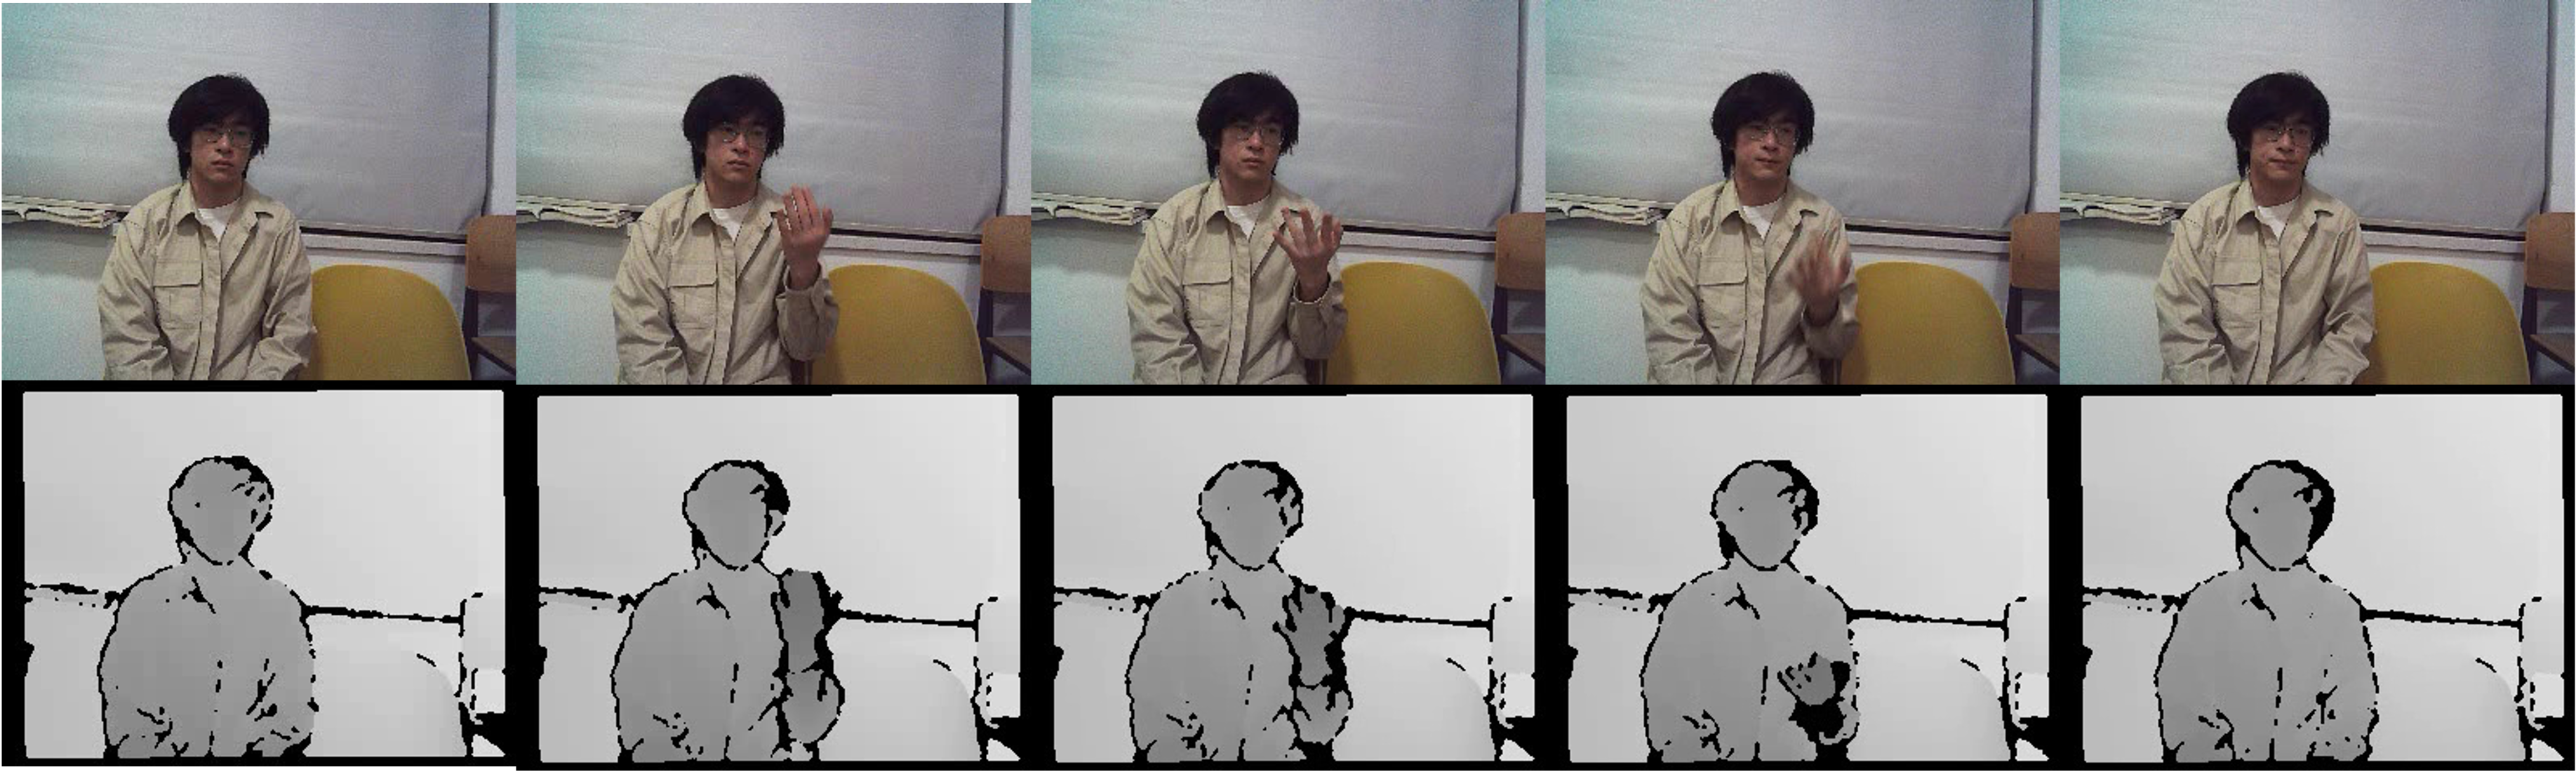
\includegraphics[width=0.8\linewidth]{aobi_sample.png}
    % \caption*{}
    \caption{商业RGB-D相机自采数据集样本示例}
    \label{fig:aobi_sample}
  \end{figure}

% 目前已采集x类xx数据(数据格式)
% 测试结果
结果显示,所提出的识别算法,在RGB-D模态的识别准确率达到了99.27\%,验证了所提出方法在实际应用场景中的高效性与可靠性。

\paragraph{识别推理速度}
我们在单张RTX2080显卡上对手语识别模块进行了推理速度测试,对同一样本进行了五次测试。如图\ref{fig:time}所示,平均推理时间为83.9ms,快于基线方法\cite{范桂双2020基于S3D}所公布的96ms。这表明我们的算法模块具有高效的推理能力,能够满足实时交互需求。

\begin{figure}
  \centering
  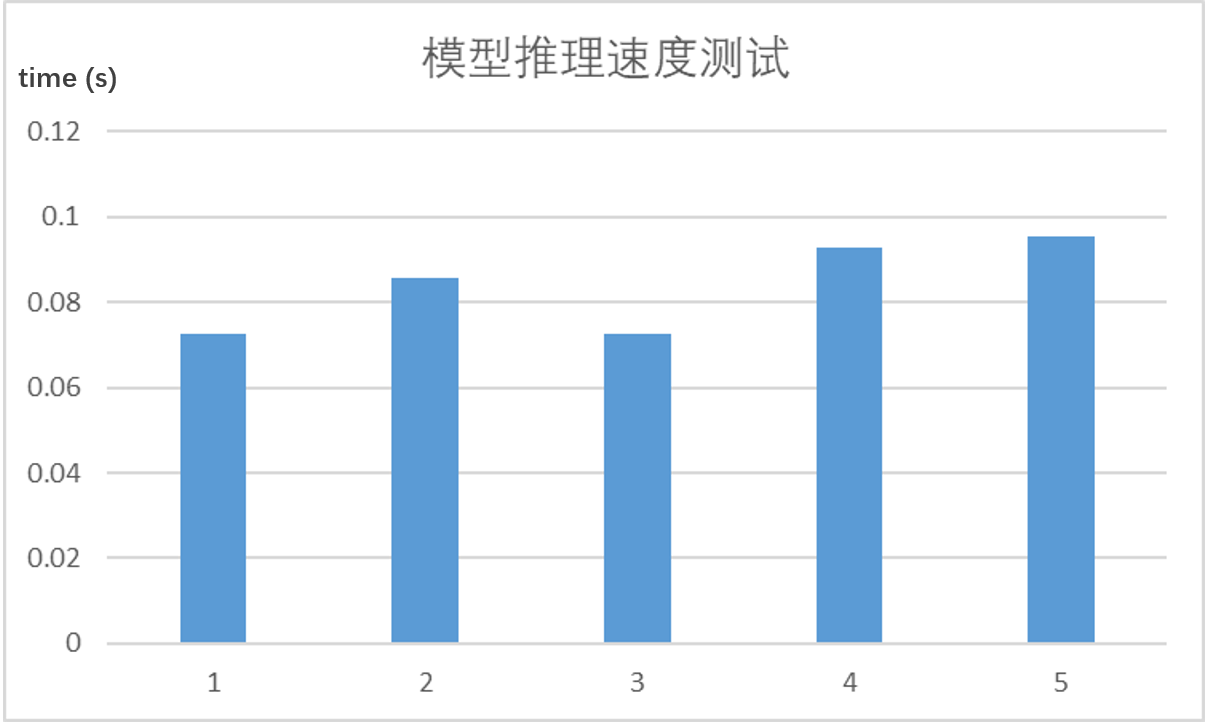
\includegraphics[width=0.65\linewidth]{time.png}
  % \caption*{}
  \caption{手语识别模块推理时间(单位:ms)}
  \label{fig:time}
\end{figure}


\paragraph{用户感知研究}
我们进行了用户研究以评估系统生成的手部动作质量。我们招募了20名参与者评估10对9秒的结果。每个生成结果从两个个方面进行评估:(i) \textit{自然度}:生成的动作与人类手势相比的真实性和自然度;(ii) \textit{匹配度}:生成的动作对给定文本描述的反映准确度。在每次评估环节中,参与者观看不同模型生成的视频片段,并针对每个方面选择表现最佳的方法。
如表~\ref{tab:perceptual_study}所示,我们的方法具有优胜的用户偏好。

\begin{table}[t]
    \centering
    \caption{手部动作生成结果的用户偏好胜率(\%)。结果表明我们生成的结果被认为更加真实和可控,在自然度和匹配度方面分别优于之前的工作~\cite{chen2024syntalker}4.65\%和1.87\%。}
    \small
    \label{tab:perceptual_study}
    \begin{tabular}{l ccc}
    \toprule
    & 自然度 & 匹配度 \\
    \midrule
    基线1~\cite{yang2024freetalker} & 20.93  & 19.38 \\
    基线2~\cite{chen2024syntalker} & 37.21  & 39.38 \\
    本文方法 & 41.86  & 41.25 \\
    \bottomrule
    \end{tabular}
\end{table}

% \subsection{用户评估实验设计}
% \textcolor{red}{
% 为全面评估系统的实际应用效果,我们设计了系统化的用户评估实验。实验招募了10名手语初学者作为测试者,实验内容包括基础手语词汇学习(10个常用手语词汇)和简单手语句子练习(5个日常用语)两个部分。
% 实验采用多维度评估指标,包括:学习效率(完成学习任务所需时间)、识别准确率(系统识别用户手语动作的准确程度)、用户满意度(基于问卷的主观评分,1-5分)以及系统可用性(基于SUS量表的评估)。实验结果显示,参与者平均用时45分钟完成全部学习任务,系统识别准确率达到92\%,用户满意度评分平均为4.3分,SUS评分为85分,表明系统具有良好的学习辅助效果和用户体验。}
    
    

    
\section{本章小结}
本章详细介绍了交互式手语学习助手系统的设计与实现。系统基于本文提出的MDSI手势识别算法和CoordSpeaker协同手势生成算法,实现了实时手语动作评估与反馈功能。通过模块化设计和高效的系统架构,成功构建了一个具有实时性、准确性和良好交互体验的手语学习辅助系统。%系统测试与用户评估结果表明,该系统能够有效辅助手语学习,具有良好的实用价值。
未来工作将进一步优化系统性能,扩展学习内容库,提升系统的实用性和适用范围。

% % % 应用
% \section{基于RGB-D手势识别的机器人导航控制系统}
% \label{sec:robot}
% 本研究拟基于所提出的 MDSI 动态手势识别算法构建一个机器人手势导航控制交互系统,并部署于奥比中光机器人平台。旨在帮助用户更好地实现机器人控制操作,同时提升手势控制过程中的人机交互体验。

% \subsection{奥比中光机器人平台}
% % 简介
% 奥比中光机器人平台(图\ref{fig:aobi_robot})是一种基于RGB-D深度视觉传感器的智能交互系统,支持实时环境感知与多模态交互能力。该平台配备高精度深度摄像头和集成式开发工具包,可捕捉手部动作的空间轨迹,进而实现多种复杂任务的导航控制与交互。

% 该平台采用主动双目结构光3D视觉传感器Gemini 2,其测试结果表明,其性能完全满足技术需求,具体包括以下参数:
% \begin{itemize}
%   \item \textbf{深度图像分辨率及帧率}:640x360@30fps,确保高质量的深度感知能力;
%   \item \textbf{测量范围}:300mm-700mm,适应多种交互距离;
%   \item \textbf{视场角}:D-FoV=99.5°@500mm,提供广阔的环境感知范围;
%   \item \textbf{测量精度}:在25\%中心区域达到0.35mm@500mm的精度,确保手势追踪的细腻与精准;
%   \item \textbf{功耗}:1.663W,支持长时间的低功耗运行;
%   \item \textbf{接口}:USB 3.0,支持高速数据传输与设备兼容性。
% \end{itemize}

% 此外,该平台的主要功能特点包括:1)\textbf{高精度深度感知}:通过RGB-D相机实现毫米级手势追踪和三维空间定位;2)\textbf{实时处理性能}:基于嵌入式硬件和深度学习推理加速,支持快速的手势识别与响应;
% 3)\textbf{灵活的扩展性}:支持多种机器人设备接口协议,可广泛应用于导航、巡逻、助理服务等场景。
% Gemini 2的优秀性能和平台的多模态交互能力,为机器人导航控制提供了高效、可靠的技术支持。


% \begin{figure}[htbp]
%   \centering
%   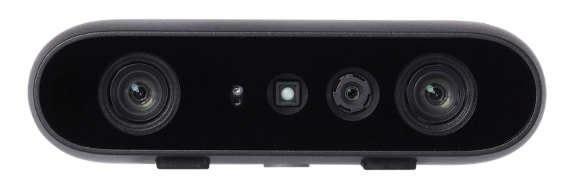
\includegraphics[width=0.7\textwidth]{gemini2.png}
%   \caption{奥比中光产品主动双目结构光3D视觉传感器Gemini 2正视实物图。}
%   \label{fig:aobi_robot}
% \end{figure}

% \begin{figure}[htbp]
%   \centering
%   \begin{subfigure}{0.7\textwidth}
%     \centering
%     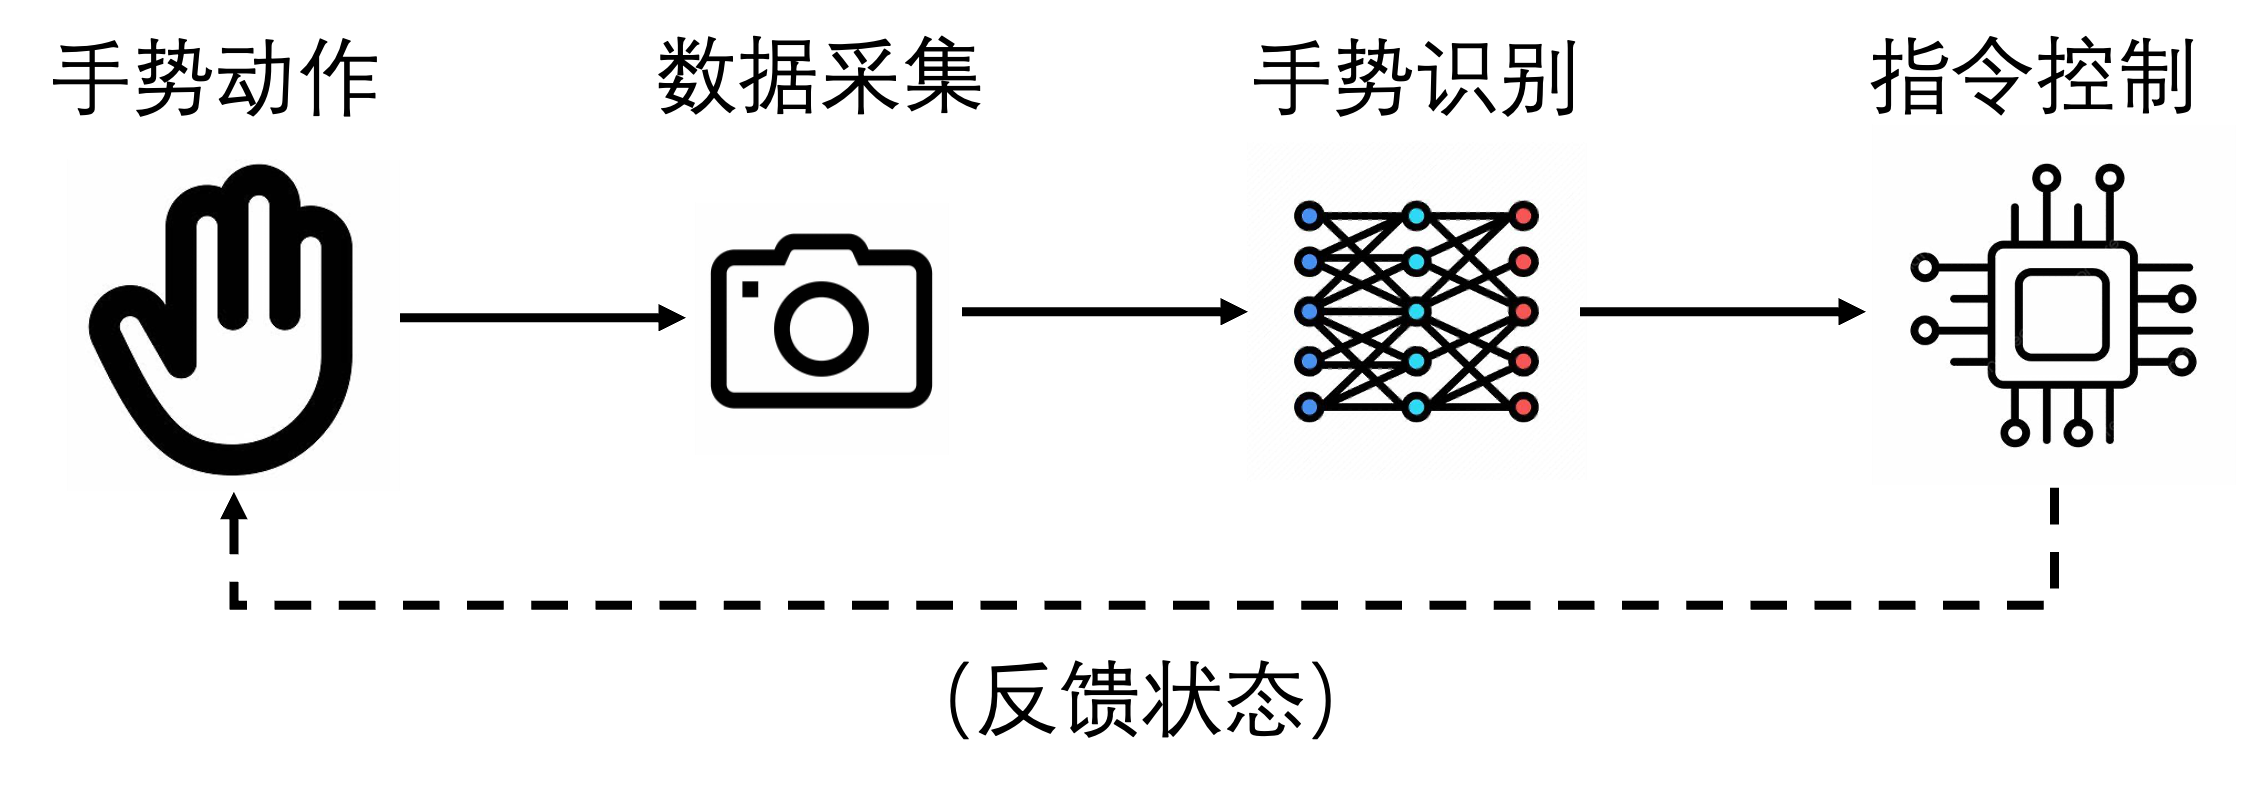
\includegraphics[width=\textwidth]{arch.png}%{system.png}
%     \caption{}
%     \label{fig:nav_control_ui}
%   \end{subfigure}
%   \hfill
%   \begin{subfigure}{0.8\textwidth}
%     \centering
%     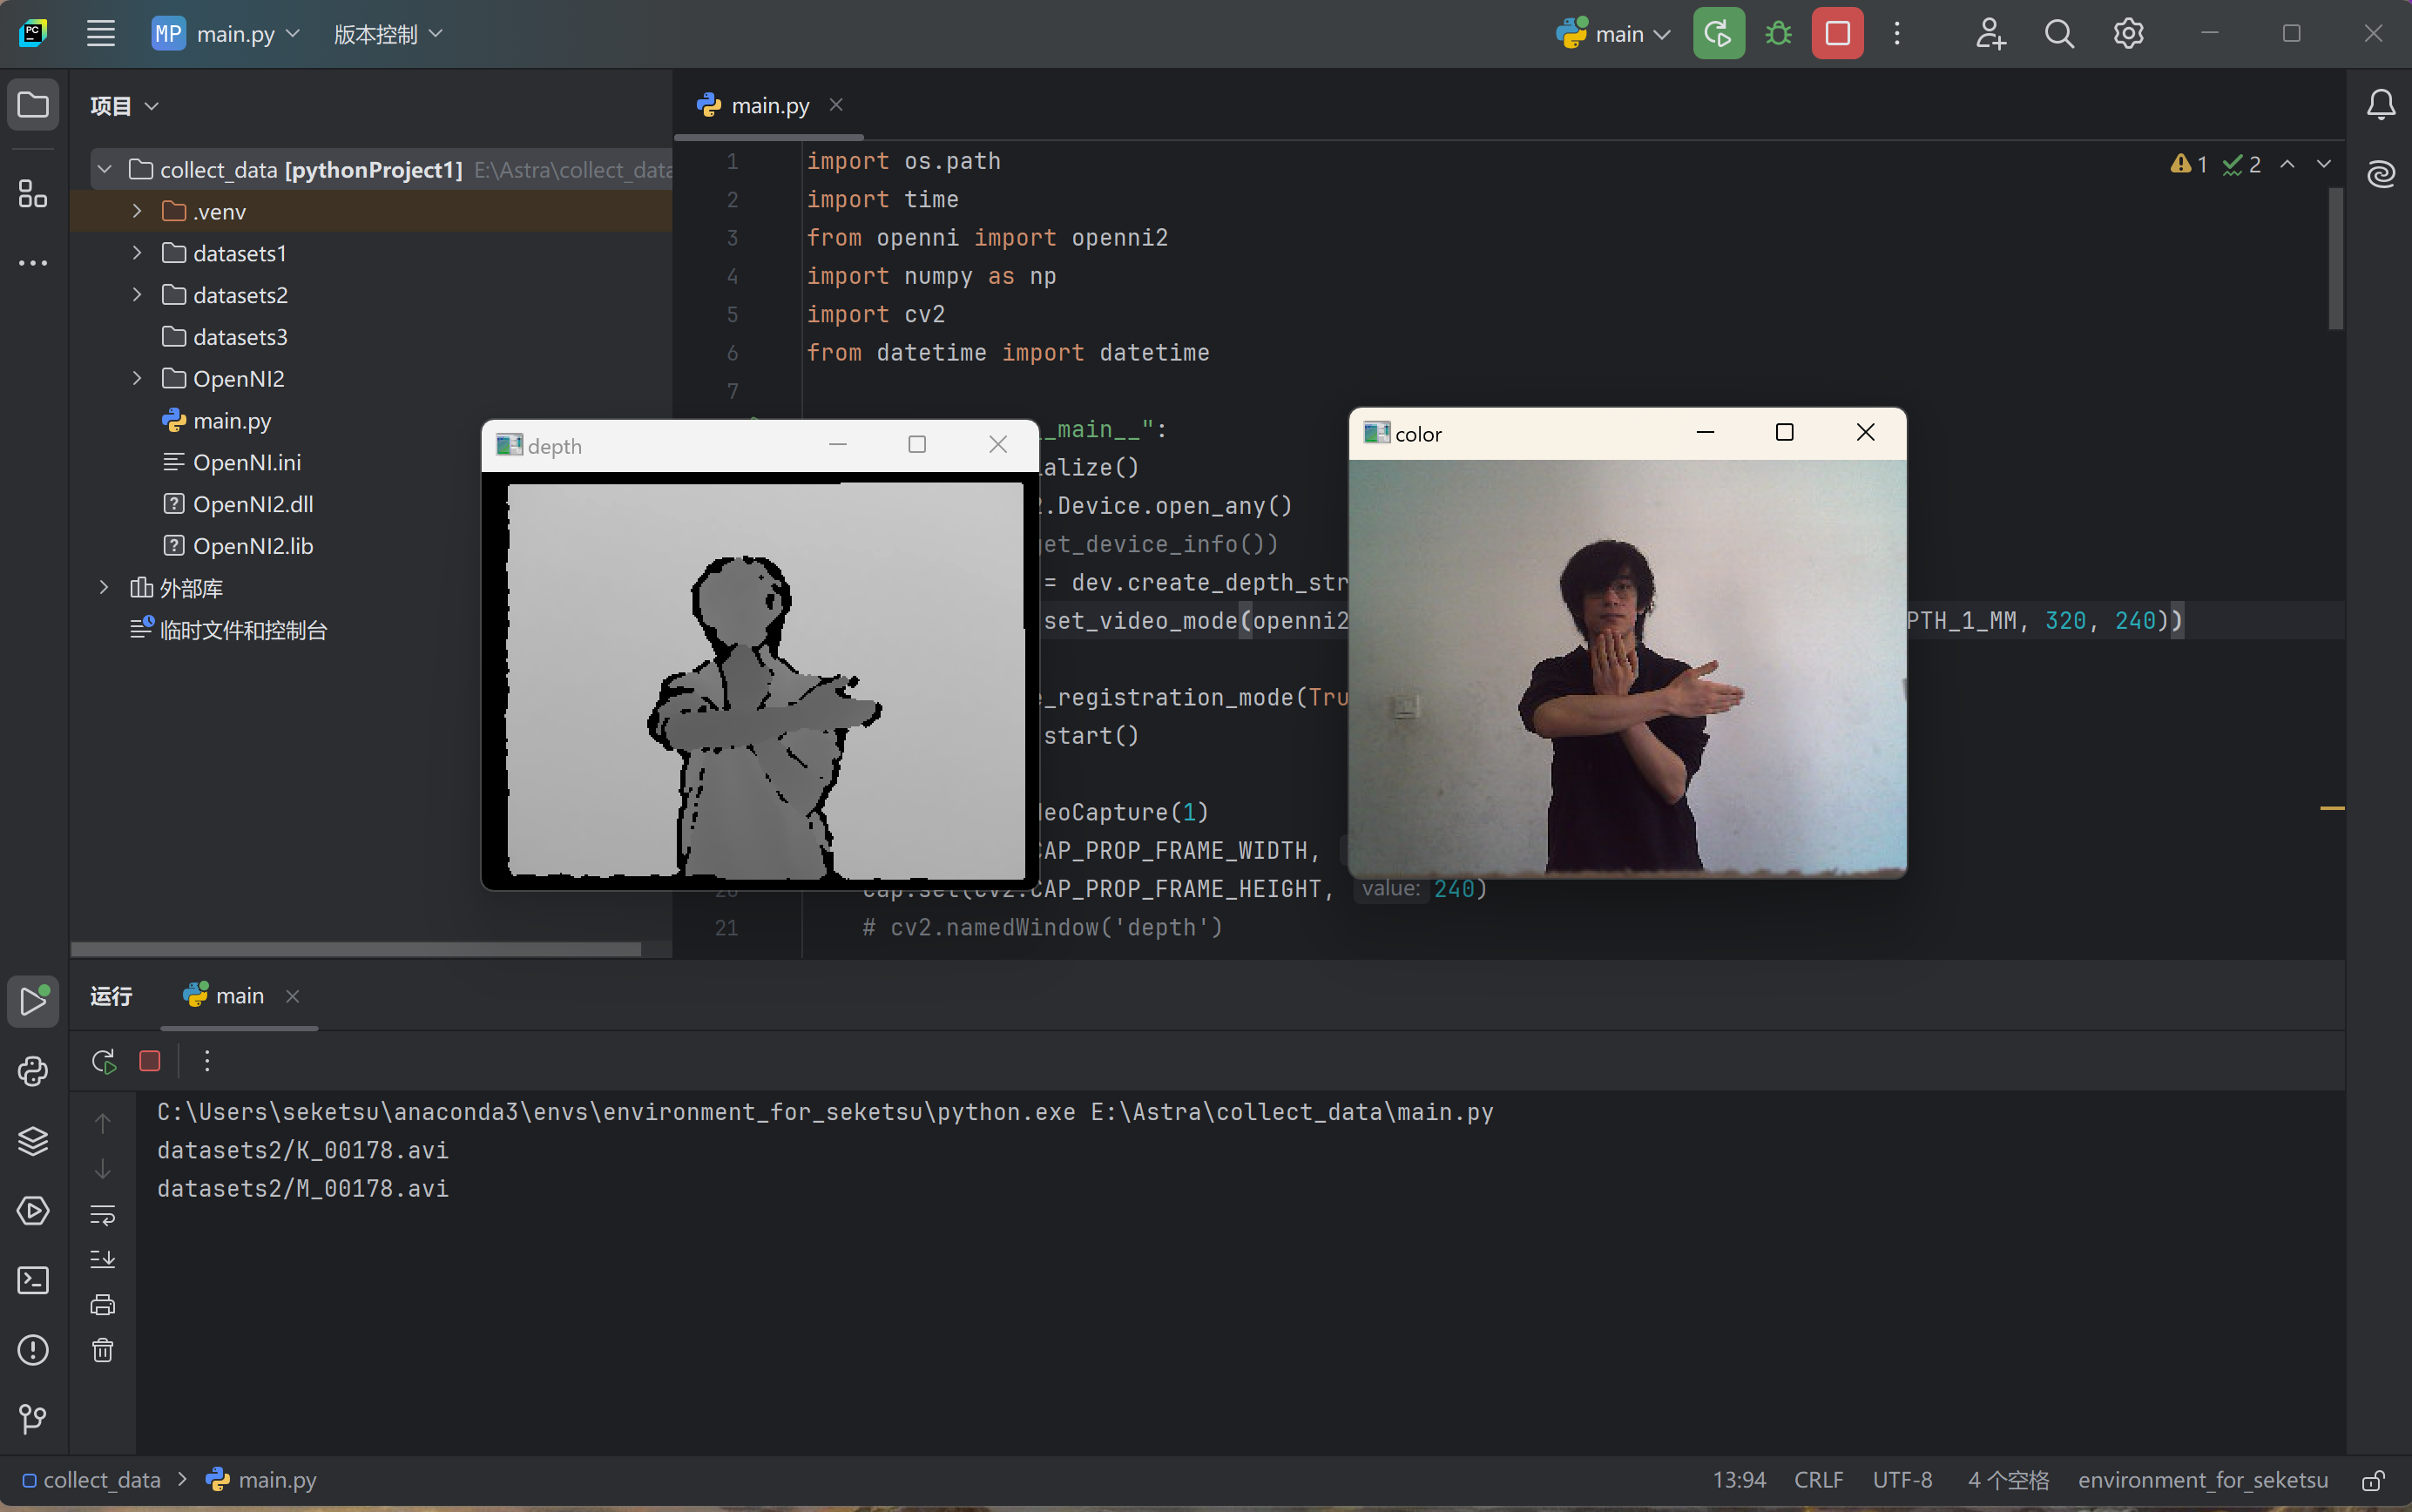
\includegraphics[width=\textwidth]{collect-min.png}%{prototype.png}
%     \caption{}
%     \label{fig:data_collection_ui}
%   \end{subfigure}
%   \caption{手势导航控制系统架构。(a)手势导航控制应用原型,(b)手势数据采集工具界面。}
% \end{figure}

% \subsection{手势导航控制应用}
% % 原型图
% 为了实现基于MDSI动态手势识别算法的机器人导航控制功能,本文设计了一个完整的手势导航控制系统(图\ref{fig:nav_control_ui}),涵盖手势数据采集、手势识别与指令生成以及机器人控制三个关键阶段。  
% \begin{enumerate}
%   \item \textbf{手势数据采集}:本研究首先开发了一款手势视频采集工具,用于录制和存储用户执行的各种手势动作。该工具具有直观的操作界面,支持实时预览和手势标签标注功能。用户在指定区域内完成手势动作,系统将采集的视频数据存储为RGB-D格式,%并附带时间戳和空间坐标信息,
%   便于后续训练与分析。图\ref{fig:data_collection_ui}展示了手势数据采集工具的界面截图,其中包括实时相机预览窗口、手势类别选择按钮,以及数据保存路径设置模块。  
%  \item \textbf{手势识别与指令生成}:通过MDSI算法对采集的RGB-D手势数据进行实时处理,系统可精准解析用户意图并生成对应的导航指令(如"向前移动"、"左转")。该模块采用高效的多模态融合策略,确保在复杂背景下的高识别率。  
%   \item \textbf{机器人控制}:解析后的手势指令通过通信接口传递给机器人平台,用于导航控制。机器人在执行过程中实时反馈状态信息(如位置、速度),以便用户随时调整指令。  
% \end{enumerate}



% 为了展示基于MDSI动态手势识别算法的实际应用效果,本文设计了一个机器人导航控制应用原型。用户通过手势控制机器人完成基本的导航任务,例如向前、向后、左转、右转、停止等。原型设计如下:

% \begin{enumerate}
%   \item 系统架构:
%   \begin{itemize}
%     \item RGB-D相机捕获用户手势信息,通过MDSI算法实时识别并解析手势指令。
%     \item 系统将解析后的手势指令传递给机器人,通过平台接口控制其移动。
%   \end{itemize}
%   \item 交互逻辑:
%   \begin{itemize}
%     \item 用户在指定区域内执行手势动作,系统显示实时反馈以确认手势识别结果。
%     \item 用户可随时更改手势指令,以调整机器人的行进路径。
%   \end{itemize}
%   \item 界面原型:包含实时摄像头画面、手势识别反馈、机器人位置状态等模块。
%   \begin{itemize}
%     \item 实时摄像头画面:展示用户手势动作。
%     \item 识别结果与指令反馈:在中央显示当前识别到的手势及对应的指令(如"向前移动")。
%     \item 机器人状态面板:右侧显示机器人位置、速度及电池状态信息。
%   \end{itemize}
% \end{enumerate}
% 以下为原型设计图:

% 以下为数据采集界面截图:




% \section{\textcolor{red}{增强现实环境下的实时手语翻译系统设计}}

% 本研究拟构建一个增强现实(AR)环境下的实时手语翻译系统,基于所提出的多流解耦手势识别算法搭建实时手语翻译应用,并部署于可穿戴AR眼镜。旨在帮助手语者更好地表达自己并维护自己的权益,同时提升手语沟通过程中的人机交互体验。
% \subsection{实时手语翻译算法管线}
% 实时手语翻译算法管线包括手语识别(SLR)和手语翻译(SLT)两个阶段\cite{chen2022two}。图\ref{fig:SLRSLT}进一步阐述了SLR与SLT的作用:与手势识别相似的,手语识别 (SLR) 旨在将输入的手语视频转录为注释序列;而手语翻译 (SLT) 直接预测给定手语视频的文本,大多数方法通过使用视觉编码器作为标记器来提取视觉特征并将其转发到翻译网络以生成口语文本,从而将该任务表述为神经机器翻译(NMT)问题\cite{chen2022two}。
% 我们使用所提出的多流解耦注意力模型作为SLR网络,并计划使用具有出色手语翻译性能的mBART\cite{liu2020multilingual}作为我们的SLT网络。
% 为了获得满意的结果,我们使用在手势识别任务上预训练好的SLR网络,并基于手语翻译数据集CSL-Daily联合微调SLR与SLT。
% 连续手势的分割是使用基于先验知识(手的放下与抬起)的手部检测进行的。
% 图\ref{fig:SLRpipe}展示了我们的实时手语翻译算法管线。
% \begin{figure}
%   \centering
%   \subcaptionbox{SLR与SLT的阐释\cite{chen2022two}\label{fig:SLRSLT}}
%     {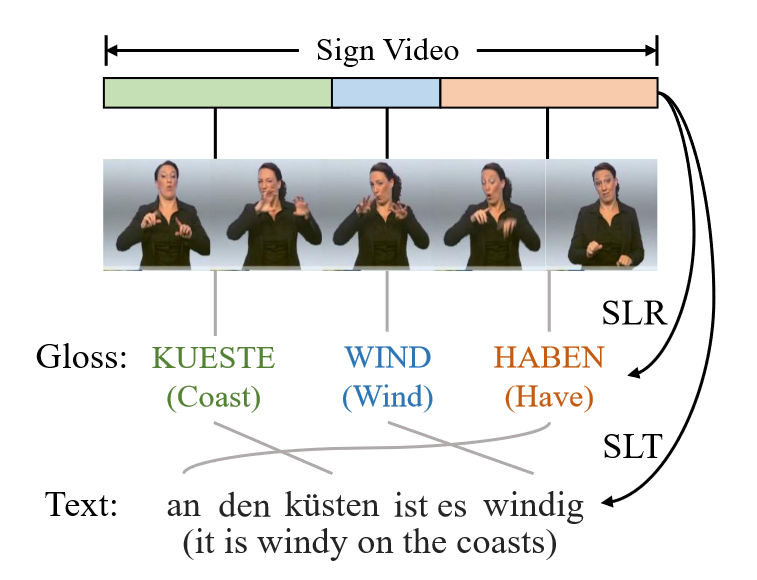
\includegraphics[width=0.5\linewidth]{SLRSLT.png}}
%   \subcaptionbox{实时手语翻译算法管线\label{fig:SLRpipe}}
%     {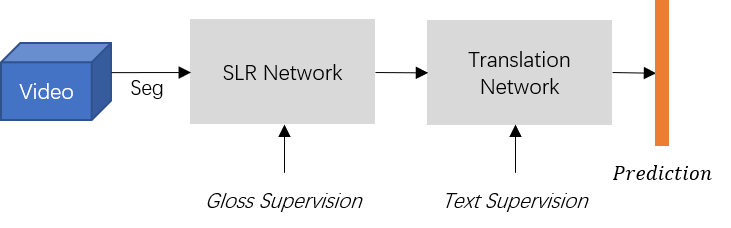
\includegraphics[width=0.8\linewidth]{SLRpipe.png}}
%   \caption{AR实时手语翻译系统原型}
%   \label{fig:SLRpipeline}
% \end{figure}

% \subsection{AR实时手语翻译应用原型设计}
% \begin{figure}
%   \centering
%   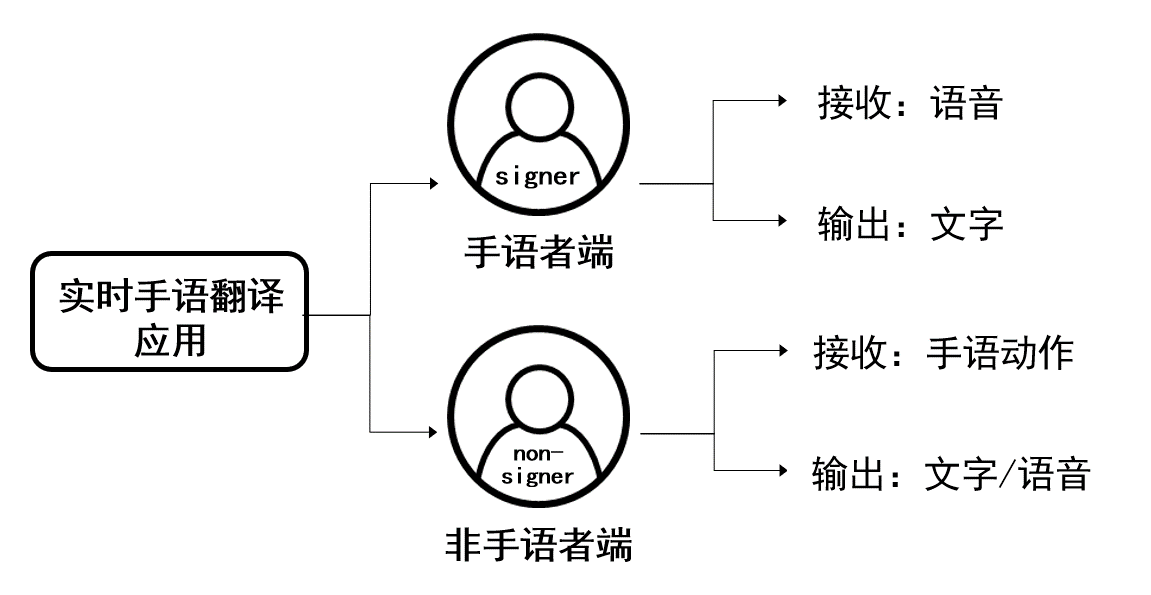
\includegraphics[width=0.8\linewidth]{system.png}
%   % \caption*{}
%   \caption{增强现实(AR)环境下的实时手语翻译系统功能设计}
%   \label{fig:system}
% \end{figure}
% 图\ref{fig:system}展示了实时手语翻译系统的基本功能设计。系统包括"手语者端"与"非手语者端":"手语者端"通过麦克风与智能语音识别API捕捉所听到的声音信号,并进行实时翻译,转换为文字显示在AR眼镜屏幕上;"非手语者端"则通过摄像头以及我们的手势识别技术,捕获手语者做出的手势动作并进行实时翻译,转换为文字显示在AR眼镜屏幕上。图\ref{fig:prototype}展示了一个简单的手语翻译系统使用场景,手语者正做出代表"Love"的手势动作,翻译所得的语义展示在AR眼镜屏幕上。

% % \begin{figure}
% %   \centering
% %   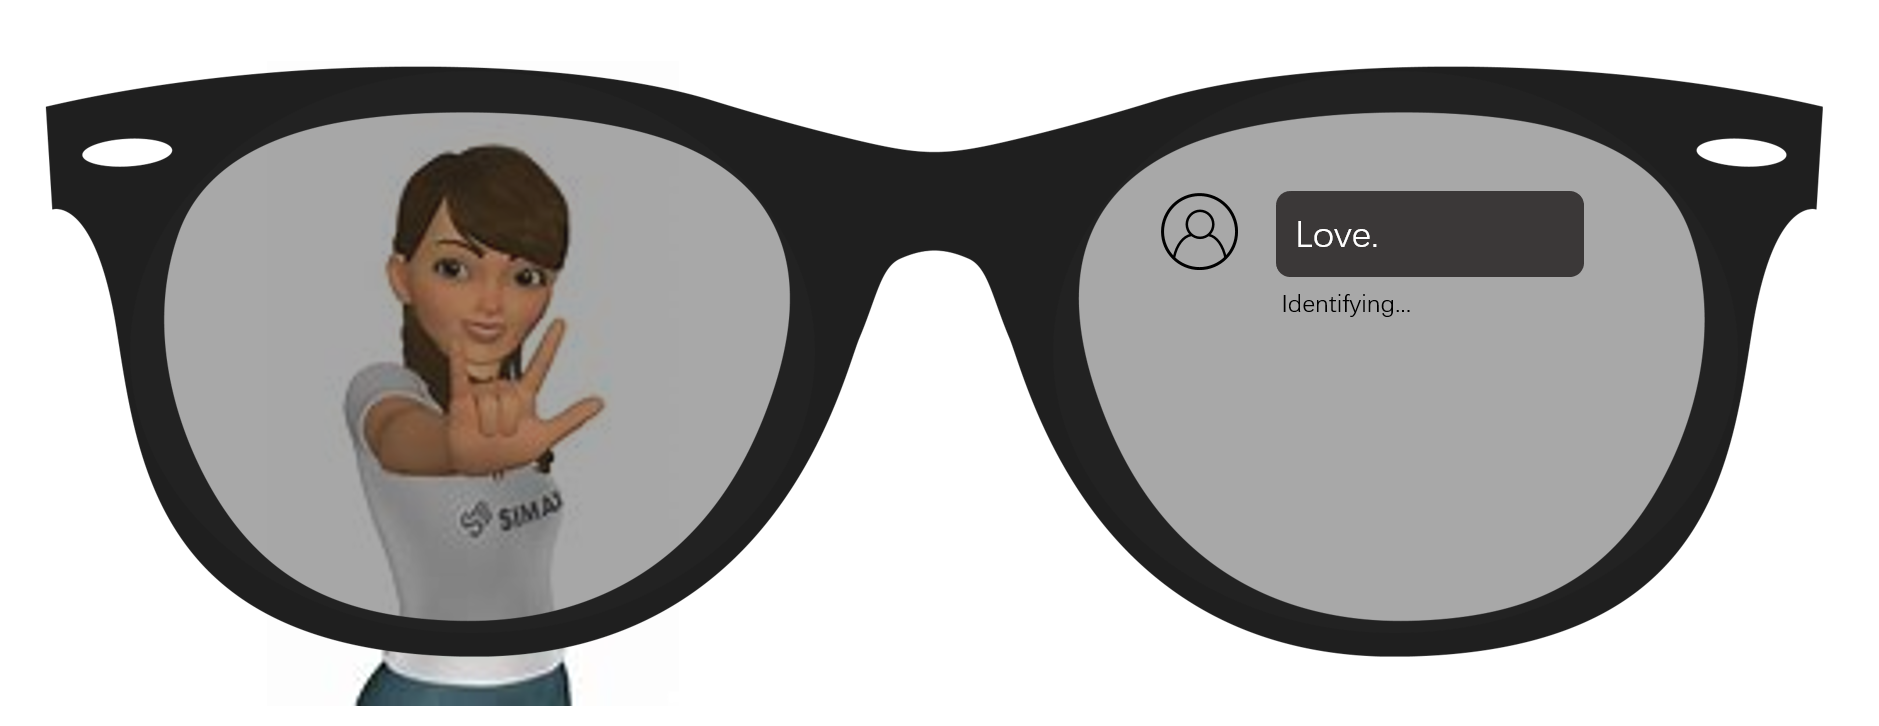
\includegraphics[width=0.9\linewidth]{prototype.png}
% %   \caption*{手语者正做出代表"Love"的手势动作,翻译所得的语义展示在AR眼镜屏幕上}
% %   \caption{一个简单的手语翻译系统使用场景}
% %   \label{fig:prototype}
% % \end{figure}

% \begin{figure}
%   \centering
%   \subcaptionbox{原型设计\label{fig:prototypea}}
%     {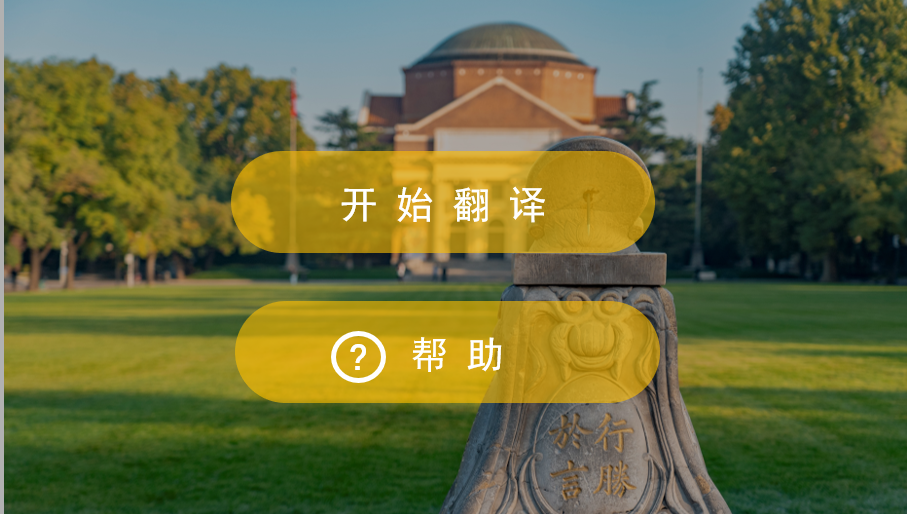
\includegraphics[width=0.65\linewidth]{prototypea.png}}
%   \subcaptionbox{使用场景示例:手语者正做出代表"Love"的手势动作,翻译所得的语义将展示在AR眼镜屏幕上\label{fig:prototypeb}}
%     {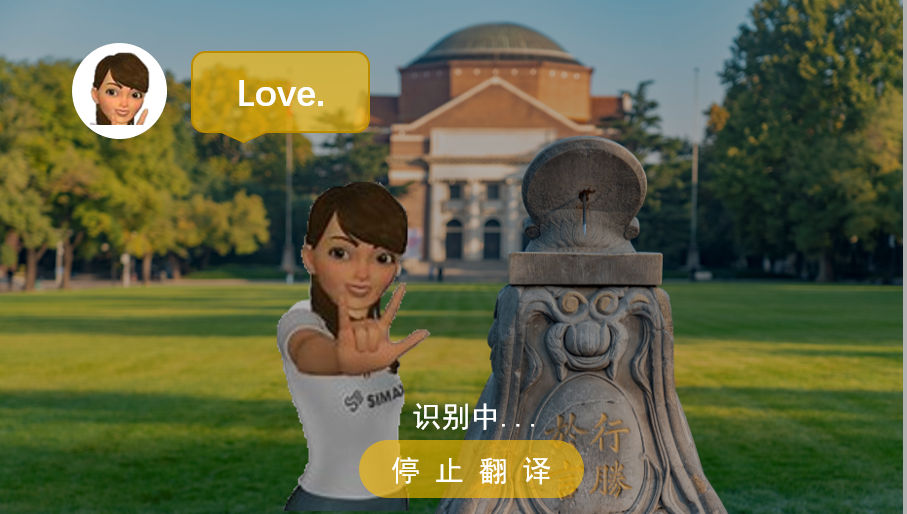
\includegraphics[width=0.65\linewidth]{prototypeb.png}}
%   \caption{AR实时手语翻译系统原型}
%   \label{fig:prototype}
% \end{figure}